Since this study is of exploratory nature, there are no predefined hypotheses we are trying to proof. The goal is rather to interpret the collected drawings and generate hypotheses from this analysis. These hypotheses will come up during the following discussion and will be highlighted. None of them were proven in any way in the context of this work, which makes them possible topics for future research. \par \medskip

The \hyperref[tb:t1]{results of task 1} show that almost two thirds of all drawings feature an explicit representation of uncertainty of some kind. This makes sense, since the task description directly asked to support the user in determining the uncertainty at a given point in time. In this context, especially graph visualizations are common. This leads us to our first hypothesis: \textbf{H1 Graph visualizations are intuitive representations to support the user in judging a specific probability value of a given point in time.} \par \medskip

Another explicit uncertainty representation we encountered multiple times is the Gradient Plot, like the one shown in Figure \ref{fig:gradSketch}. This is interesting, since \citet{gschwandtner2016visual} identified these plots to work very well for this kind of task. If the following hypothesis \textbf{H2} holds true, they indeed seem to be a very good choice for those tasks, also if the target user group encompasses non-experts. \textbf{H2 Gradient Plots are intuitive representations to support the user in judging a specific probability value of a given point in time.}\par \medskip

\begin{figure}[H]
	\begin{minipage}{.45\textwidth}
		\centering
		\captionsetup{width=0.8\textwidth}
		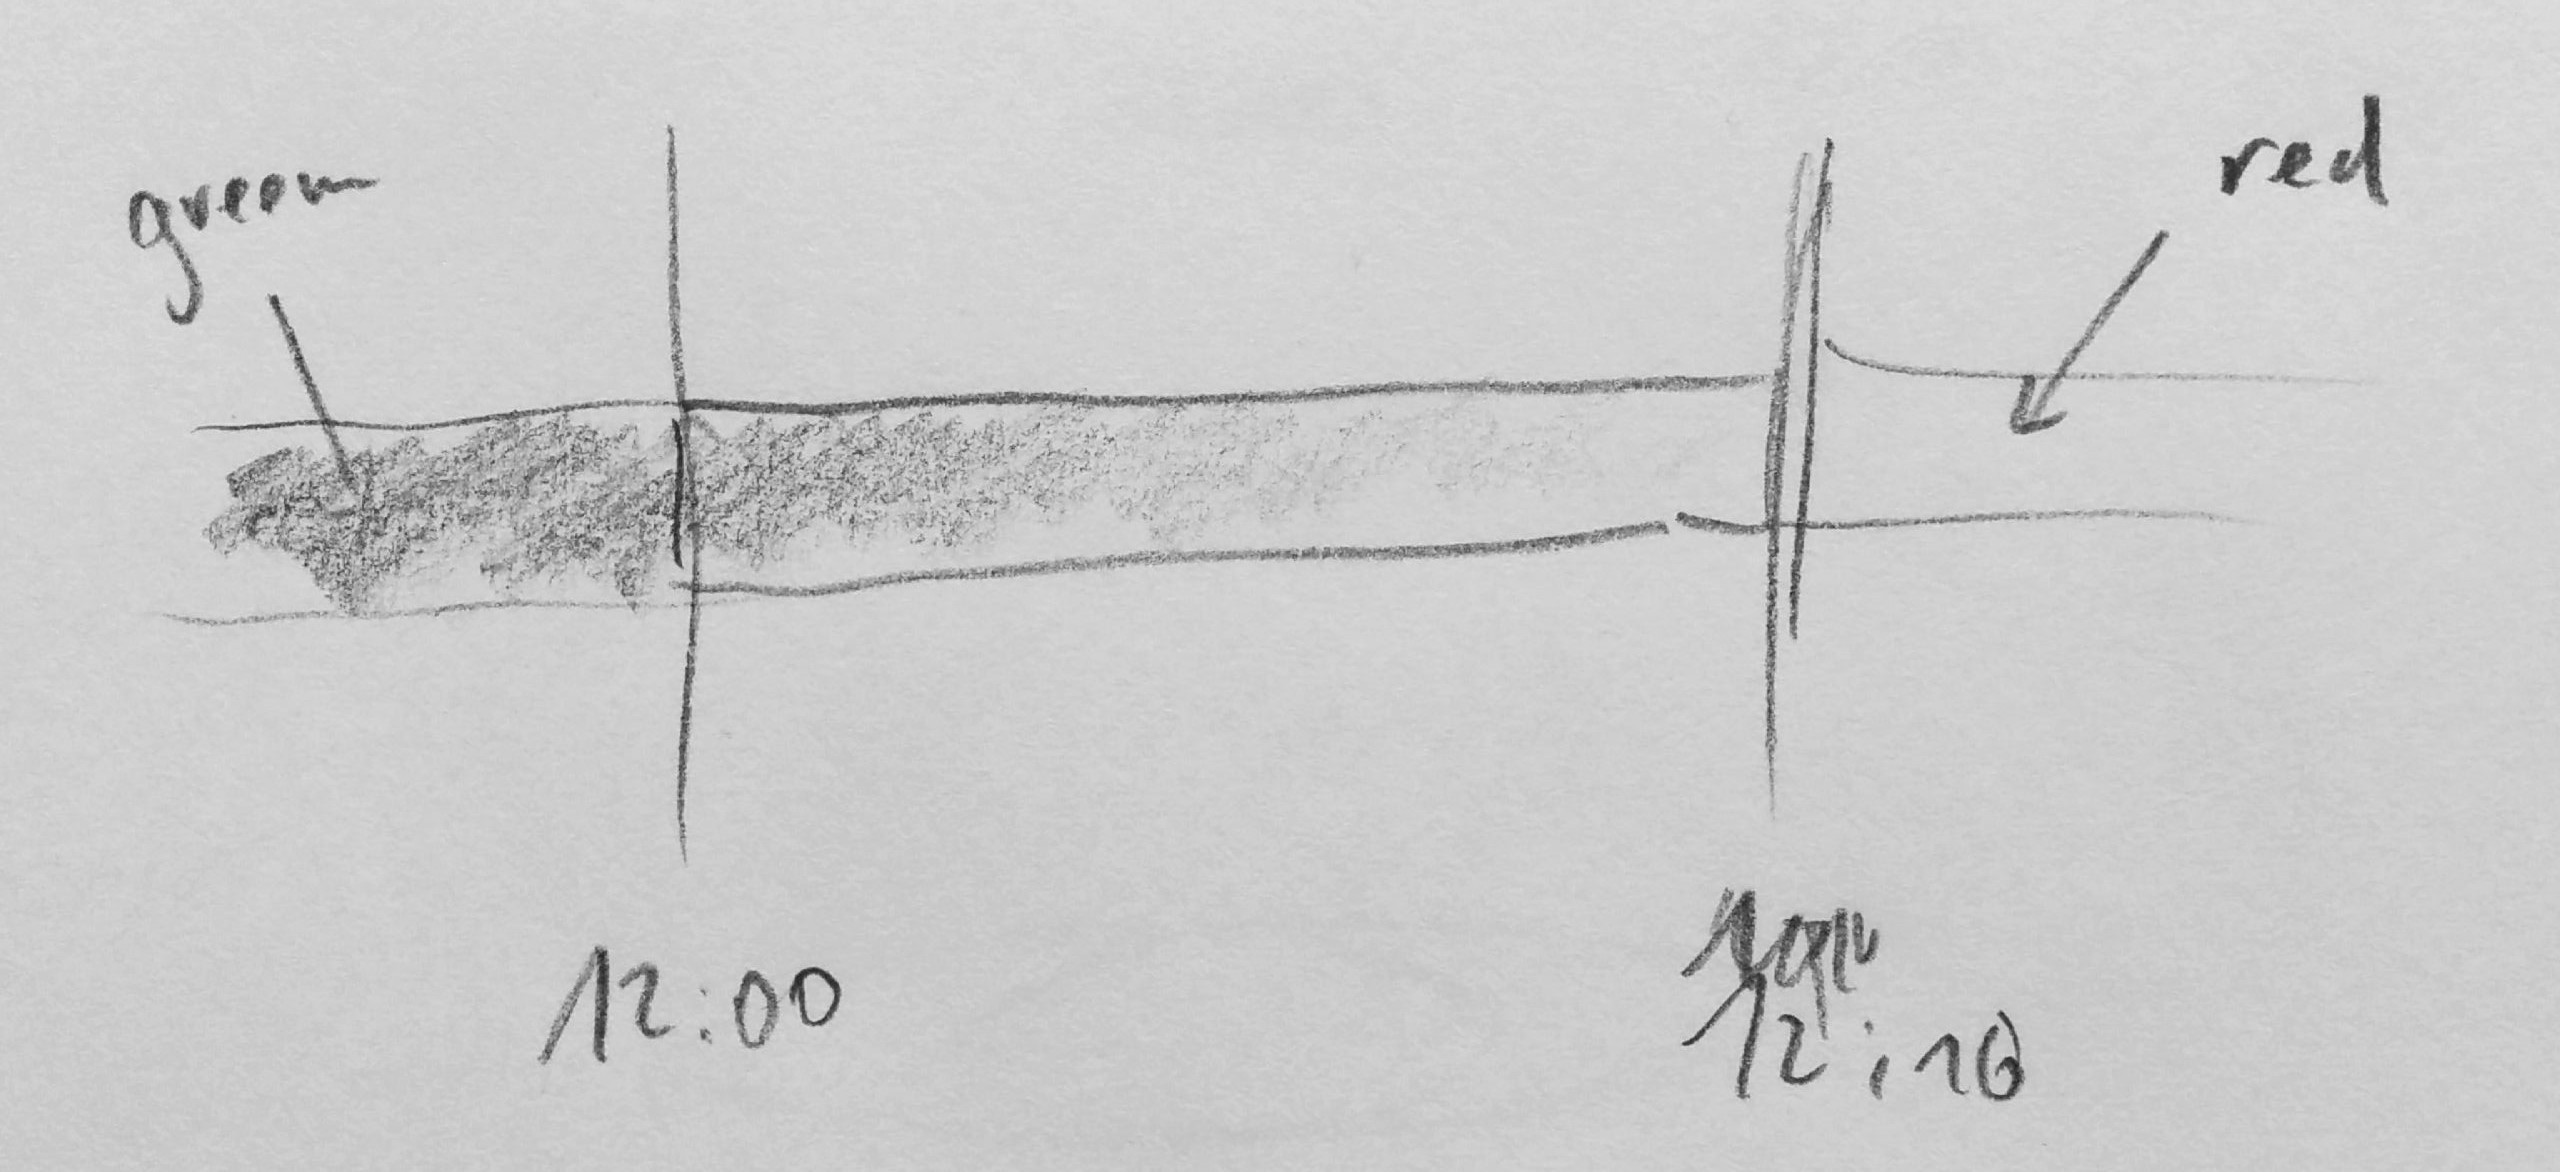
\includegraphics[height=0.5\textwidth]{figures/gradientSketch.jpg}
		\caption{\textit{This sketch utilizes a color gradient from green to red to represent the probability of a specific point in time.}}
		\label{fig:gradSketch}
	\end{minipage}
	\begin{minipage}{.55\textwidth}
		\centering
		\captionsetup{width=1.0\textwidth}
		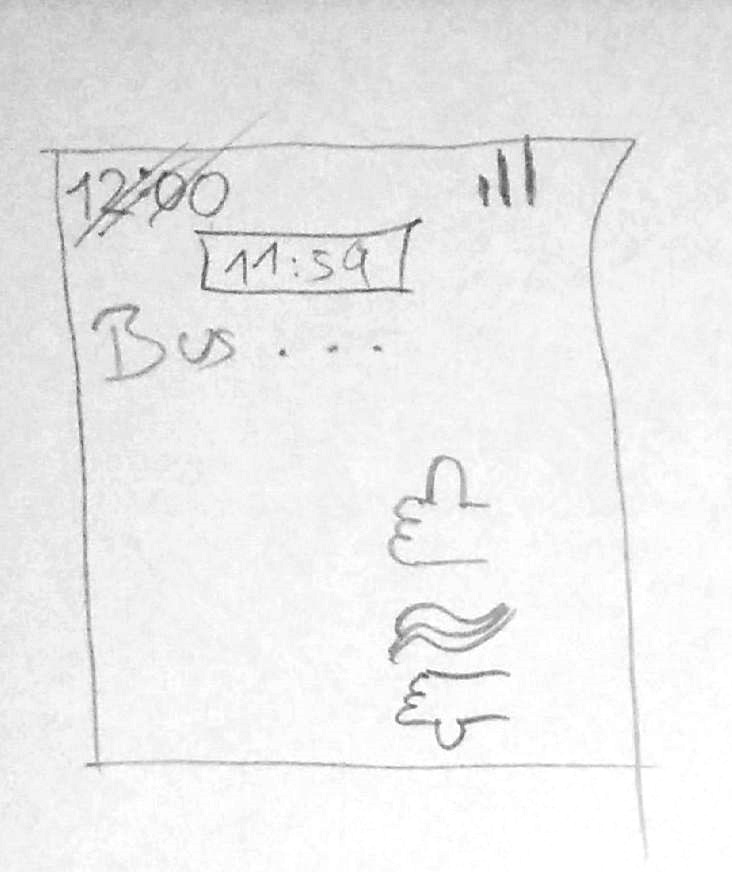
\includegraphics[height=0.55\textwidth]{figures/iconSketch.jpg}
		\caption{\textit{In this design the participant worked with user interaction and icon representations. The user has to enter a point in time and receives an icon, representing the corresponding probability, as feedback.}}
		\label{fig:iconSketch}
	\end{minipage}
\end{figure}

Other explicit representations of uncertainty utilize icons to convey the actual probability values to the user. An example for this can be seen in Figure \ref{fig:iconSketch}. We believe this approach to be especially intuitive, but lacks the precision to represent exact values. Therefore we think: \textbf{H3 Icon representations, like smiley faces, are a good approach to represent probability values in a very intuitive way, as long as these values do not have to be judged very precisely.}\par \medskip

Even though most visualizations feature an explicit representation of uncertainty, 11 sketches, like the one in Figure \ref{fig:bounded}, are of a bounded nature, which only shows the bounds of the uncertain interval, rather than explicit values. If this is the case because this is seemed to be the best way for these participants, or if they simply had no good idea to represent uncertainty explicitly, we do not know. Either way, these representations seem to be intuitive to most people, even though they are not well suited for the task at hand. \citet{gschwandtner2016visual} showed that this approach is well suited to convey durations and temporal bounds to the user, which leads us to the following joint hypothesis: \textbf{H4 Bounded visualizations are intuitive and effective ways to convey durations and temporal bounds of events with uncertain start and end times to non-expert users.}\par \medskip

\begin{figure}[H]
	\begin{minipage}{.5\textwidth}
		\centering
		\captionsetup{width=0.8\textwidth}
		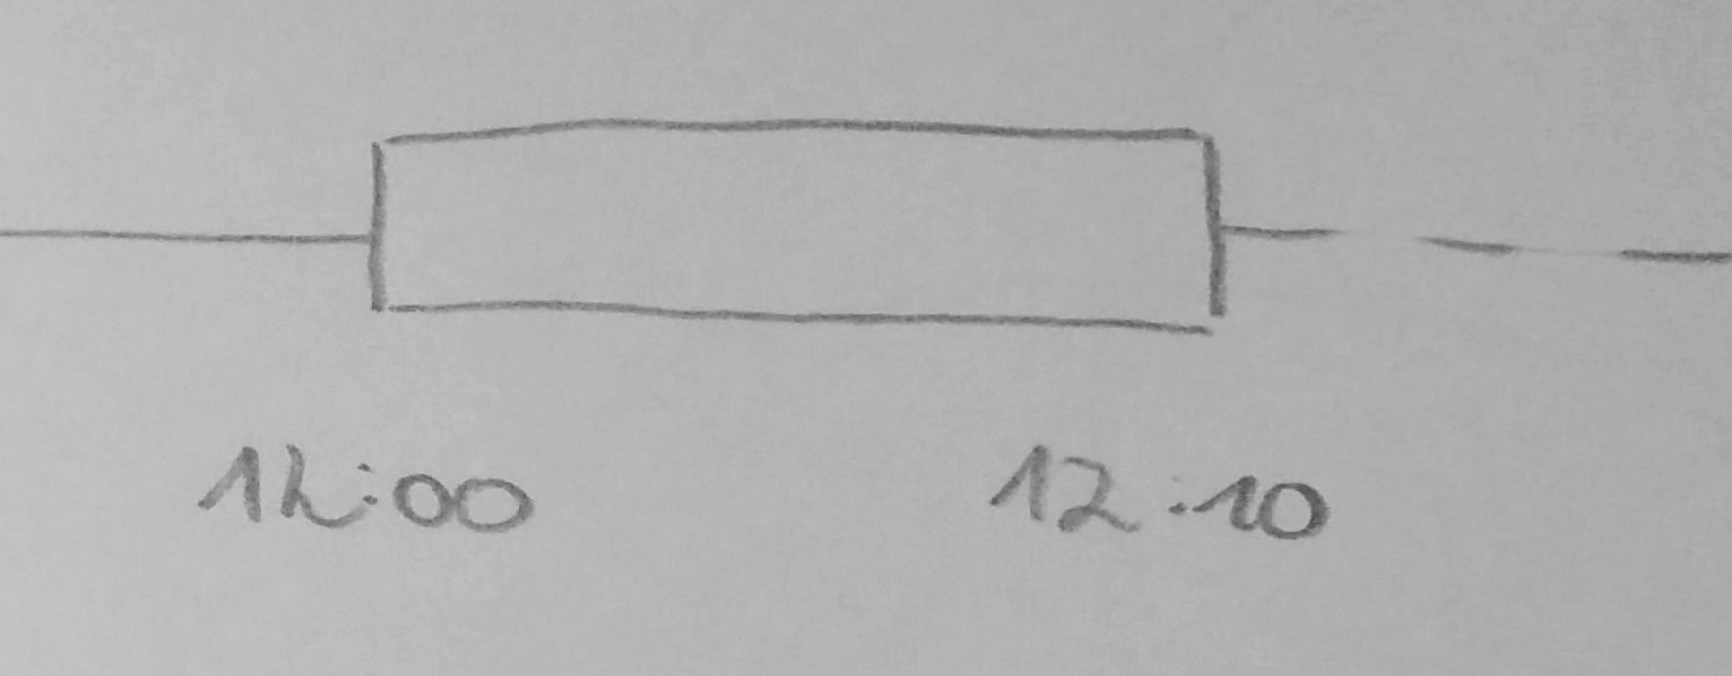
\includegraphics[height=0.35\textwidth]{figures/bounded.jpg}
		\caption{\textit{The broader part from 12:00 to 12:10 marks the uncertain part of the event, while the continuous line on the left marks the certain part.}}
		\label{fig:bounded}
	\end{minipage}
	\begin{minipage}{.5\textwidth}
		\centering
		\captionsetup{width=1.0\textwidth}
		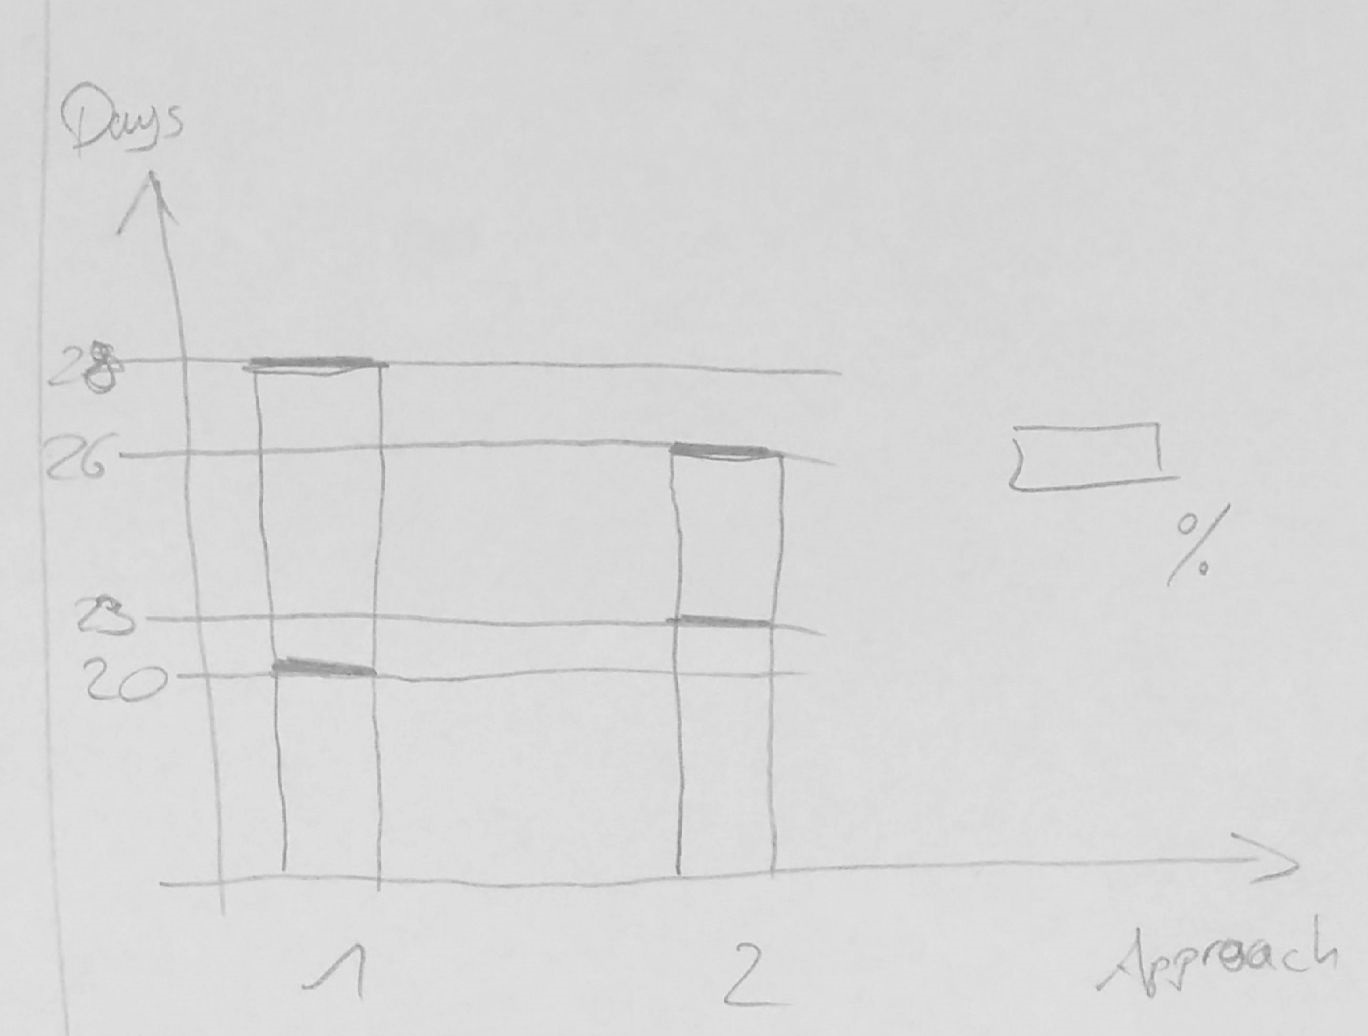
\includegraphics[height=0.6\textwidth]{figures/timeBotTop.jpg}
		\caption{\textit{In this vertical bar chart the time is mapped to the y-axis going from the bottom to the top. The two bars represent the two project approaches.}}
		\label{fig:timeBotTop}
	\end{minipage}
\end{figure}

The assumption that most people would represent time on the horizontal axis from left to right is confirmed by our results. From the total amount of 93 sketches we collected and analyzed, 80\% represented time in this way. We also assumed that time would usually be represented from top to bottom, if the time line occupies the vertical axis. This assumption was falsified, since only two sketches featured time this way. The rest of the drawings showed time either in a clockwise manner (clock metaphors) or from bottom to top, like in Figure \ref{fig:timeBotTop}. These findings indicate that the question regarding the truth of the following hypothesis can not trivially be answered: \textbf{H5 It is more intuitive to a non-expert user group to vertically map time from the bottom to the top, than vice versa.}\par \medskip


In Table \ref{tb:t23} the results of Task 2 and 3 can be seen. It shows that only five drawings feature graph representations in these tasks. We believe that this is due to the task we asked our participants to solve with their visualization. To judge the average time an event takes, people seem to prefer to see the two uncertain intervals next to each other, instead of superimposed graphs. \textbf{H6 If two or more events are compared to each other, it is more intuitive to show them in a juxtaposition, than superimposed in the same space.} This hypothesis is also supported by the numbers of superpositions (7) and juxtapositions (23) in the collected drawings. \par \medskip

Another thing that can be seen in the results table of Task 2 and 3, is that most sketches feature an explicit representation of uncertainty, but there does not seem to be one favorite way to do so. Within the collected drawings uncertainty is represented using graphs (see Figure \ref{fig:t2graph}), other representations that encoded it in length or height (see Figure \ref{fig:t2length}), through color (see Figure \ref{fig:t2color}) and through interaction (see Figure \ref{fig:t2interaction}). All of those approaches came up five times within our experiment. Hence, the results do not show any indication of one of those techniques being more intuitive than others in the context of a comparative visualization. What can be seen though, is that there was not a single icon representation used for these tasks. We believe that the reason for this is that icons do not lend themselves to comparisons, since they also do not represent single values accurately. \textbf{H7 Icon representations are not well suited for direct comparison.} \par \medskip


\begin{figure}[H]
	\begin{minipage}{.5\textwidth}
		\centering
		\captionsetup{width=0.8\textwidth}
		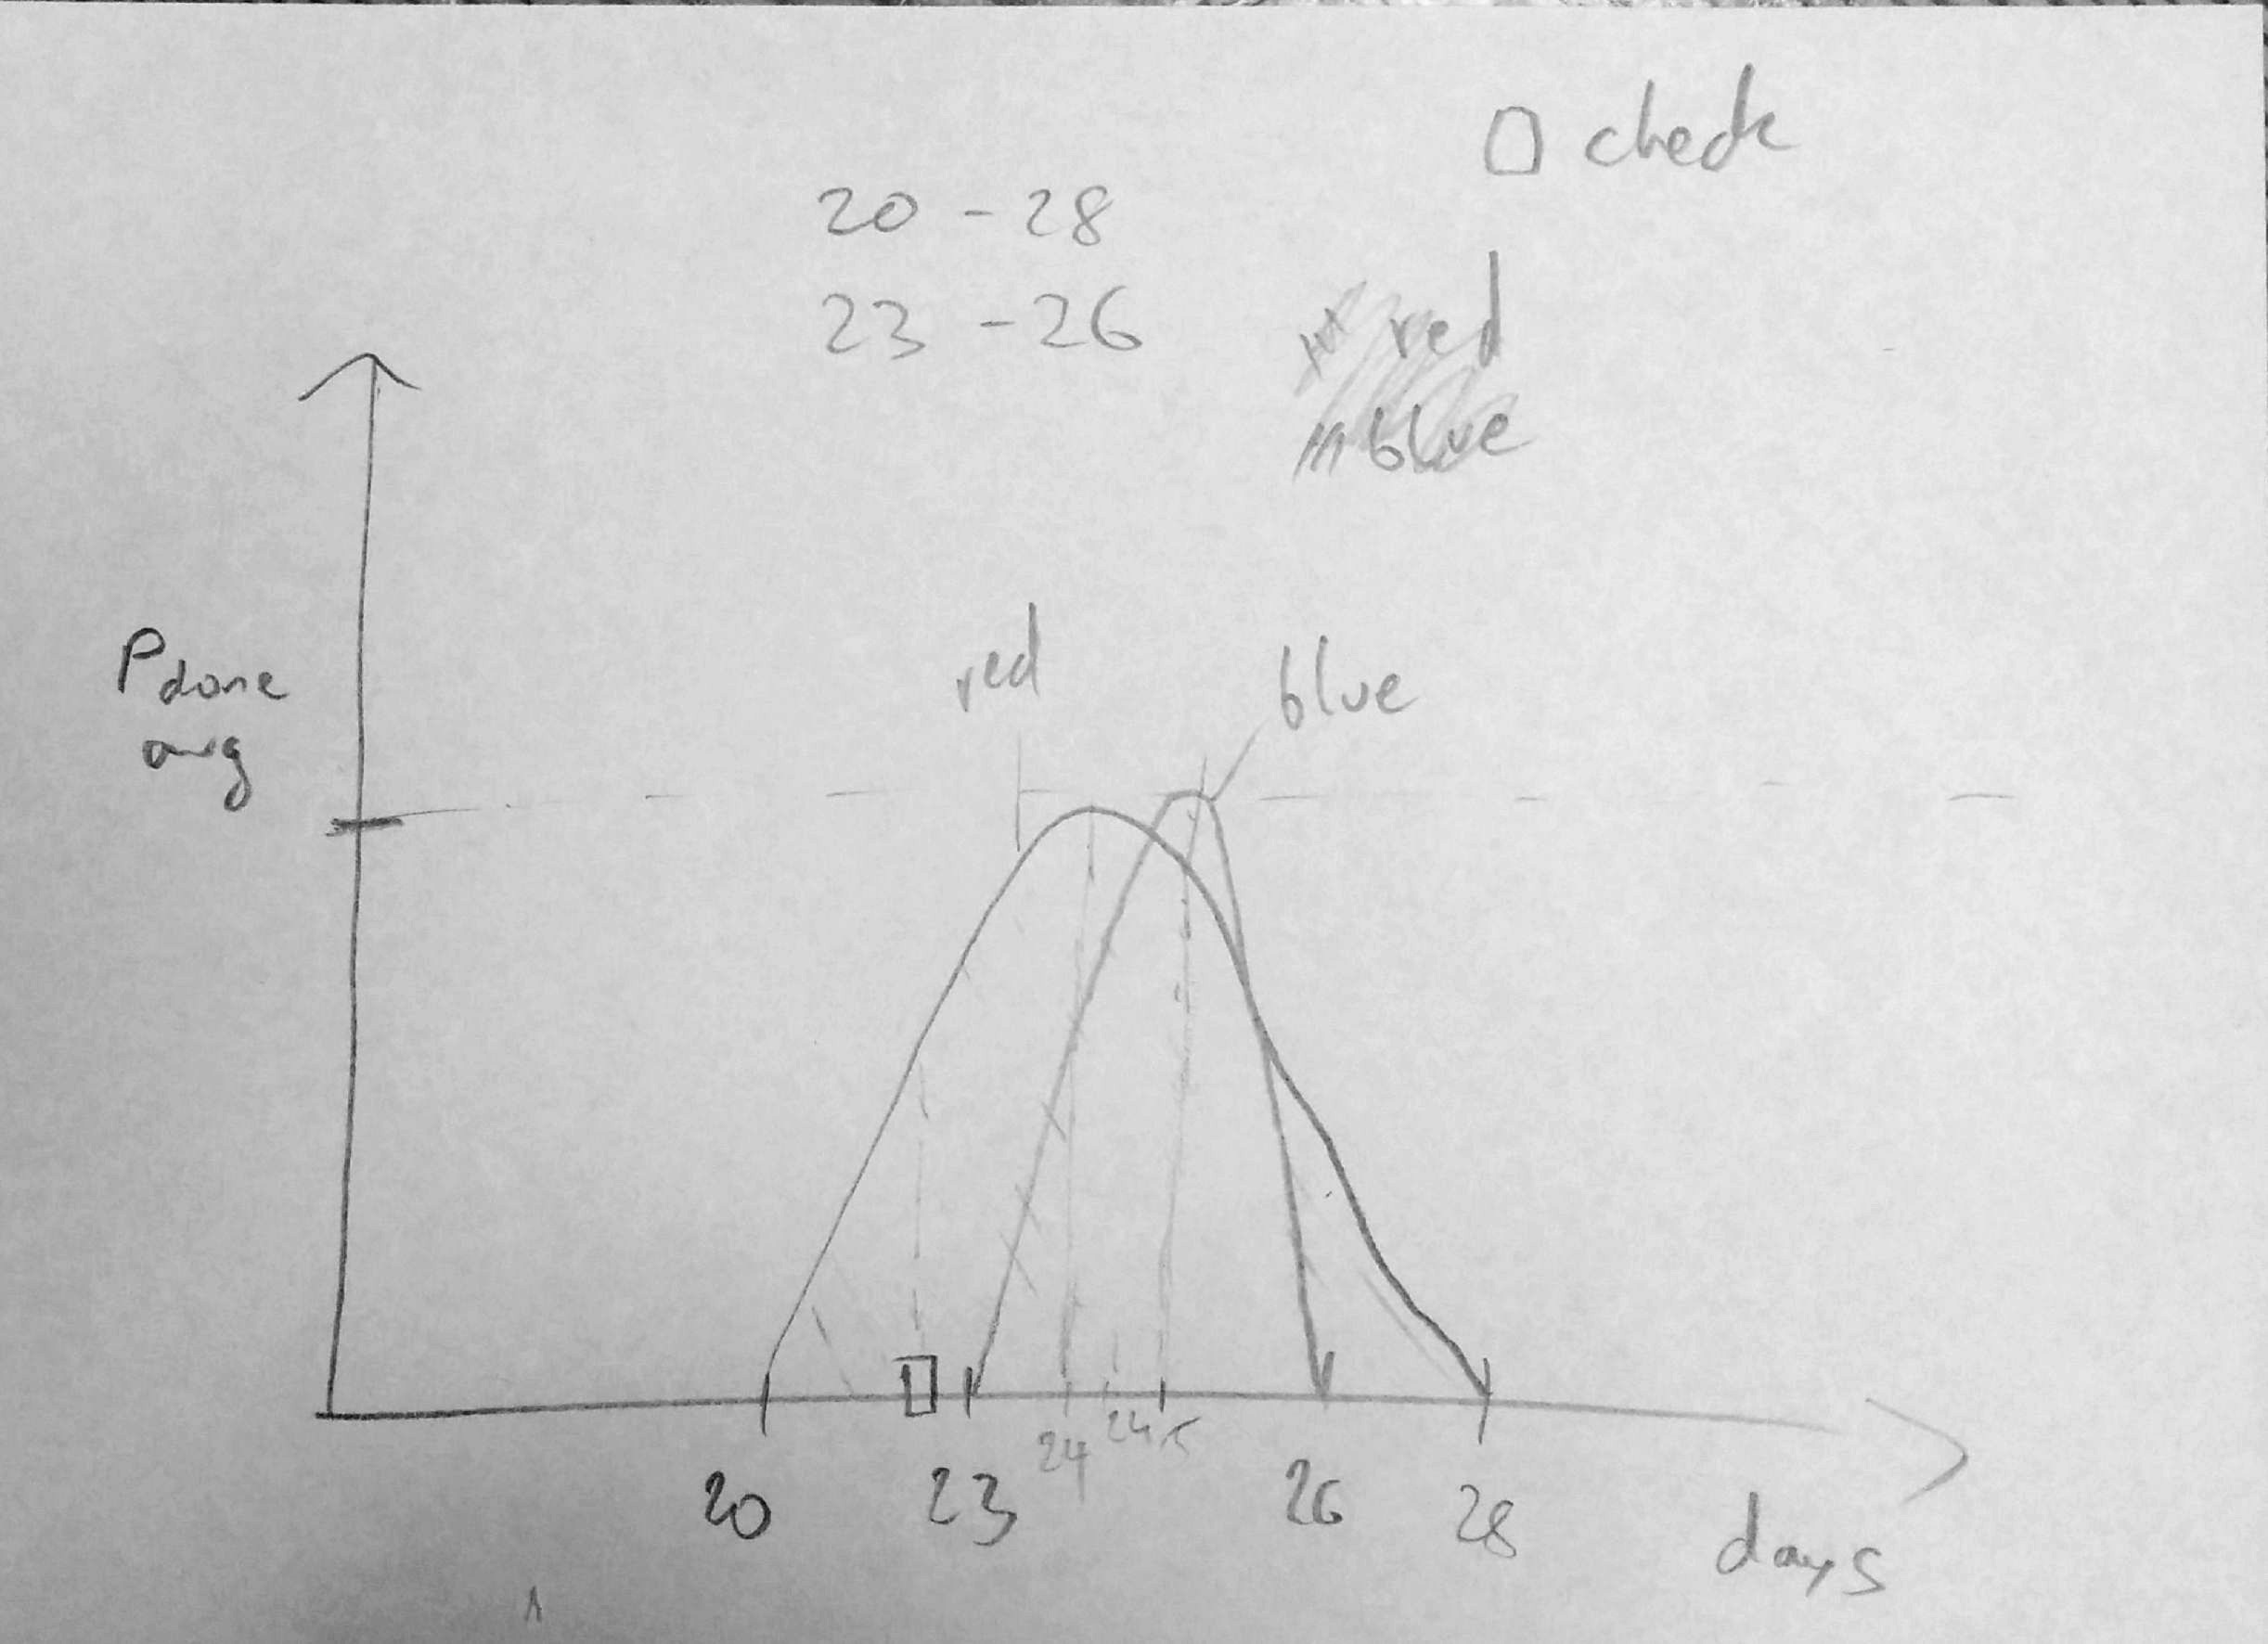
\includegraphics[height=0.5\textwidth]{figures/t2graph.jpg}
		\caption{\textit{This is a conventional graph visualization, that features two superimposed graphs. The graphs show the possibility of the event ending at the corresponding point in time.}}
		\label{fig:t2graph}
	\end{minipage}
	\begin{minipage}{.5\textwidth}
		\centering
		\captionsetup{width=1.0\textwidth}
		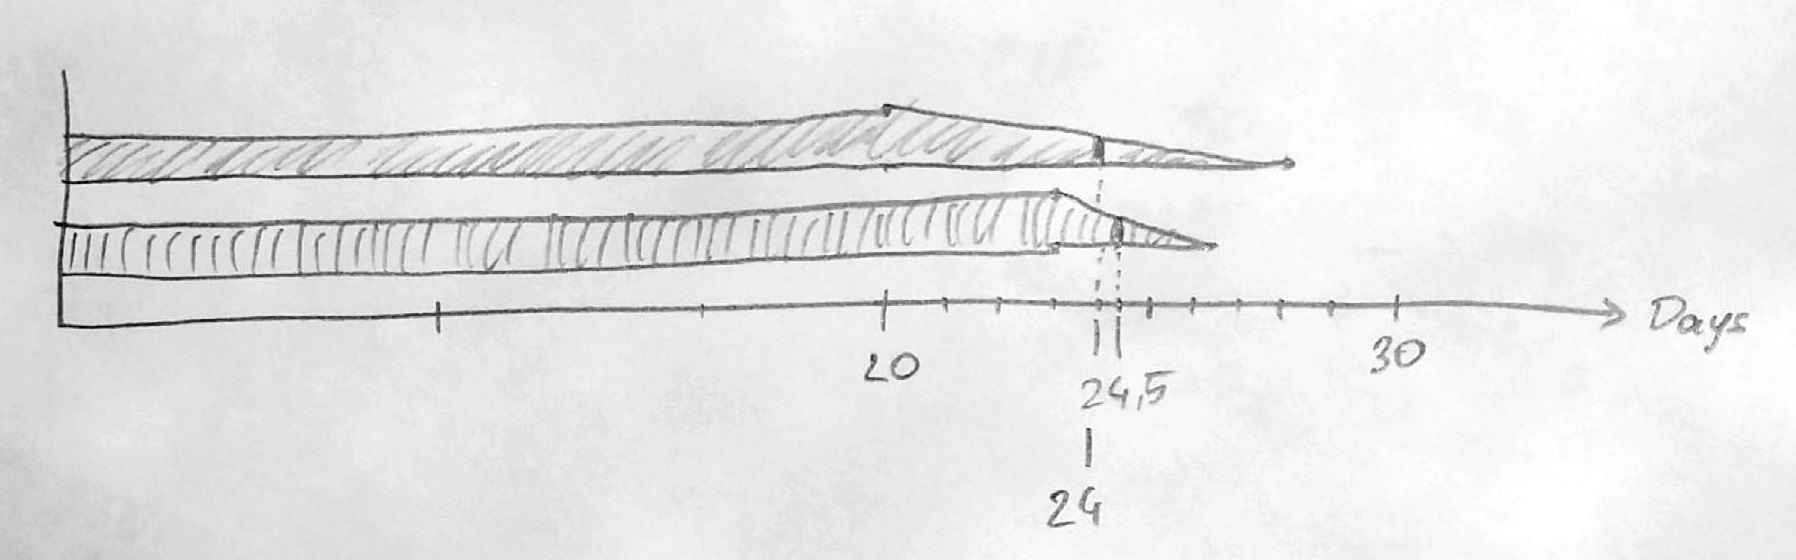
\includegraphics[height=0.33\textwidth]{figures/t2length.jpg}
		\caption{\textit{The uncertain time intervals are bounded by the sloping part of the horizontal bars. Additionally the thickness of the bar at a given point in time represents the possibility that the event is still going on at that point in time.}}
		\label{fig:t2length}
	\end{minipage}
\end{figure}
\begin{figure}[H]
	\begin{minipage}{.5\textwidth}
		\centering
		\captionsetup{width=0.8\textwidth}
		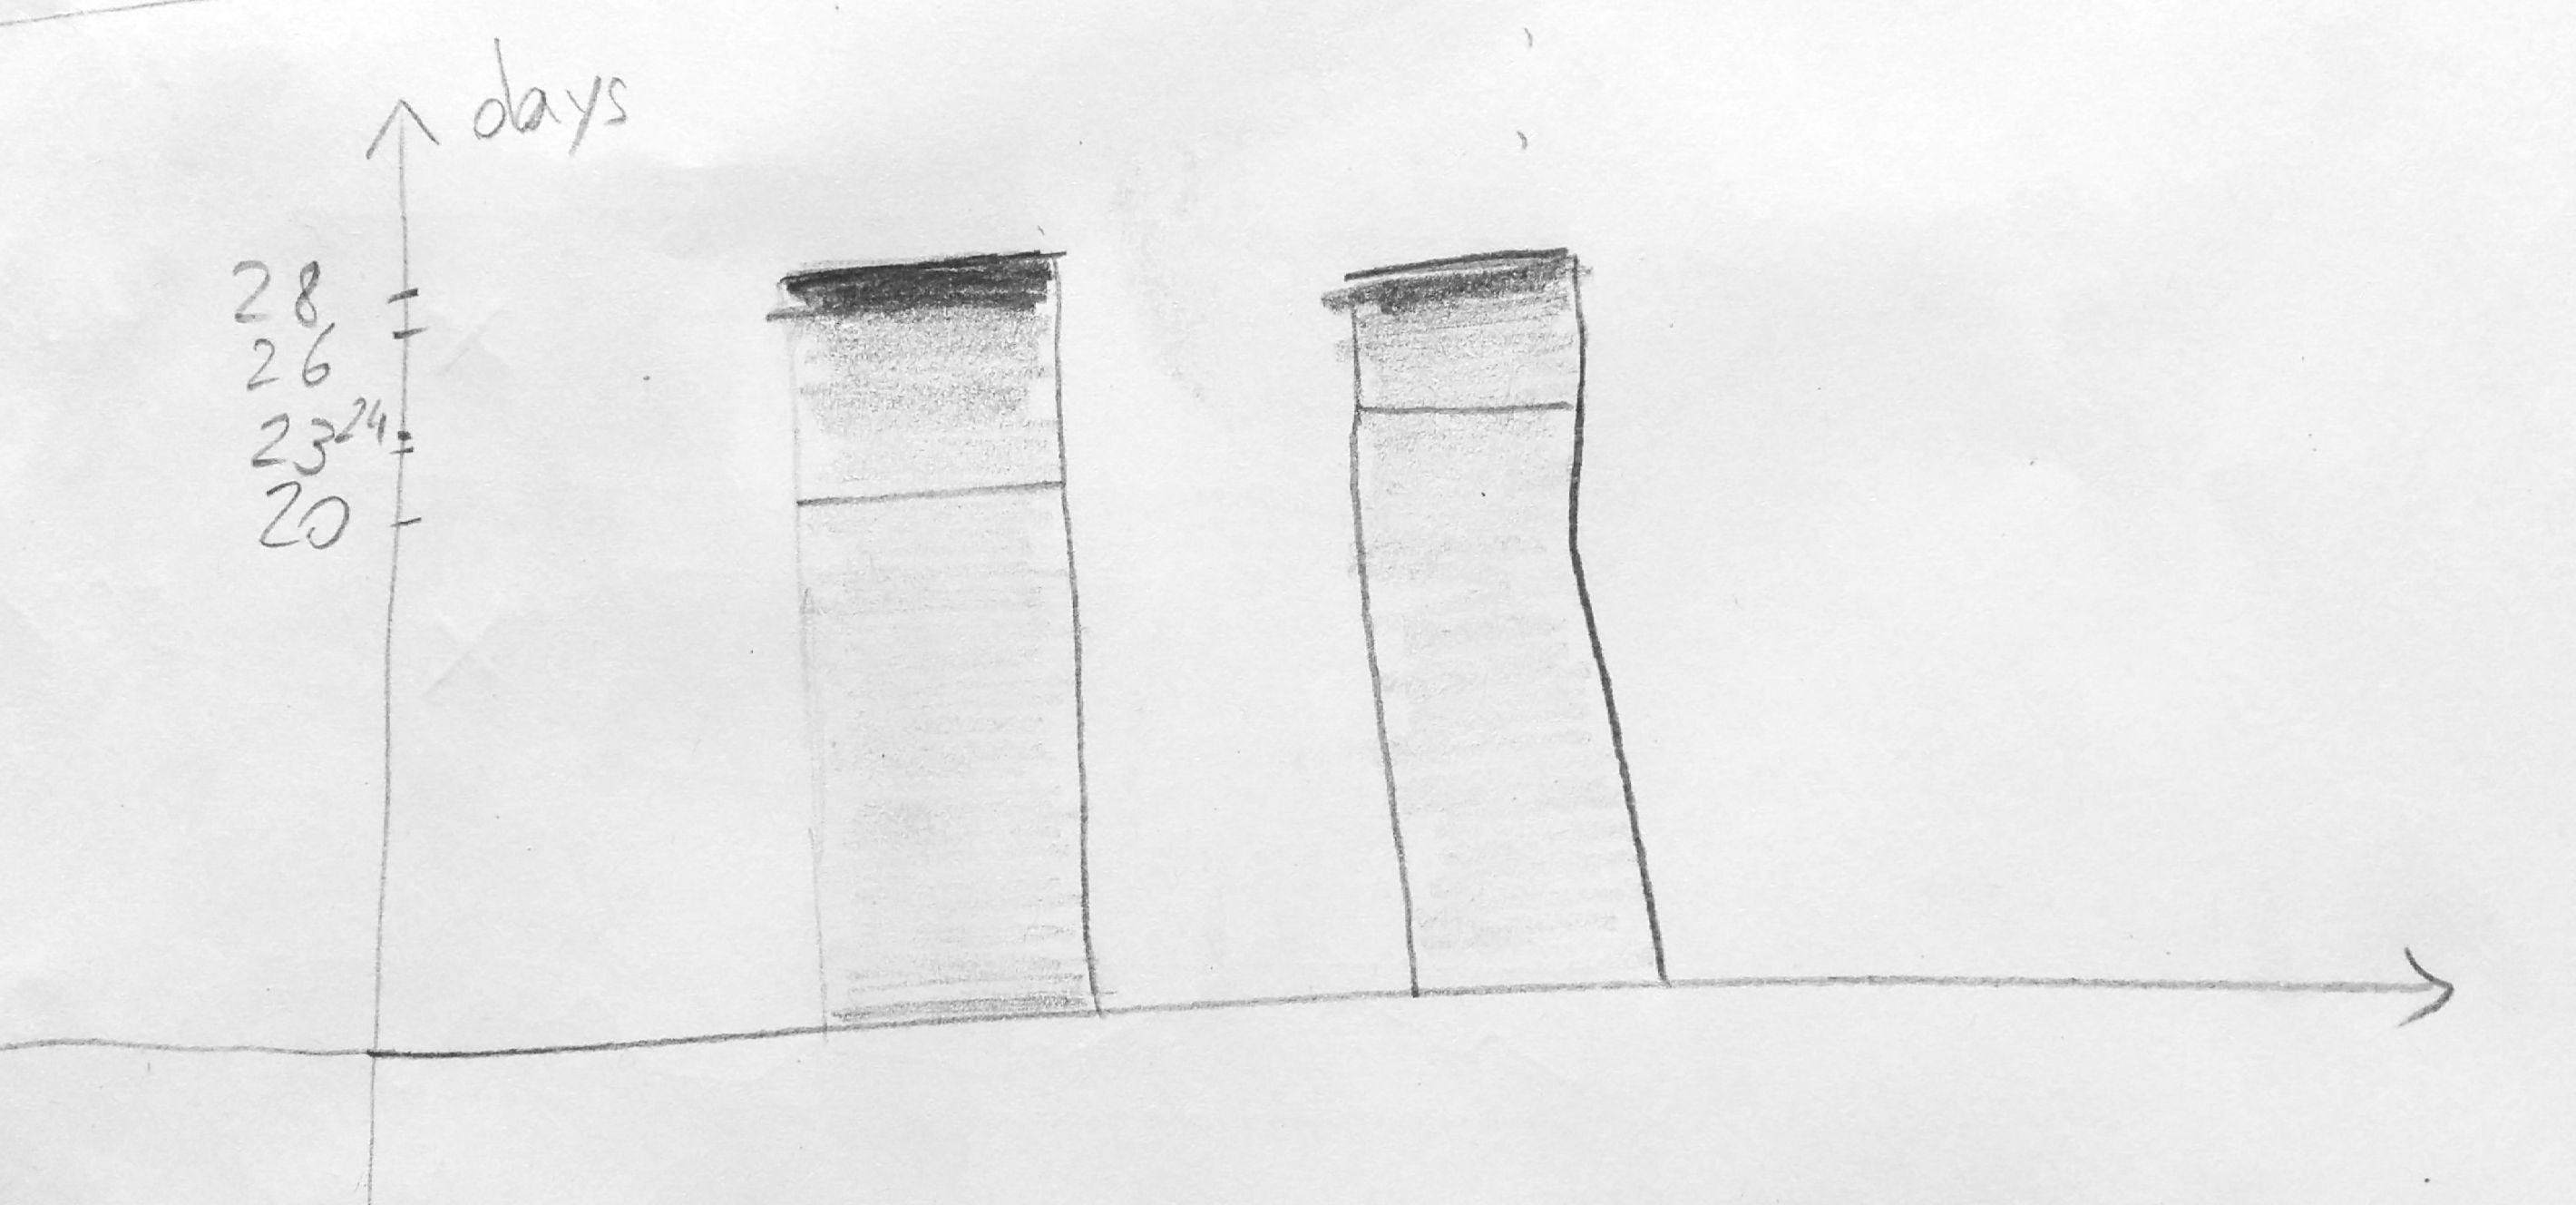
\includegraphics[height=0.4\textwidth]{figures/t2color.jpg}
		\caption{\textit{In this vertical bar chart color is used to additionally show the uncertainty explicitly for every point in time.}}
		\label{fig:t2color}
	\end{minipage}
	\begin{minipage}{.5\textwidth}
		\centering
		\captionsetup{width=1.0\textwidth}
		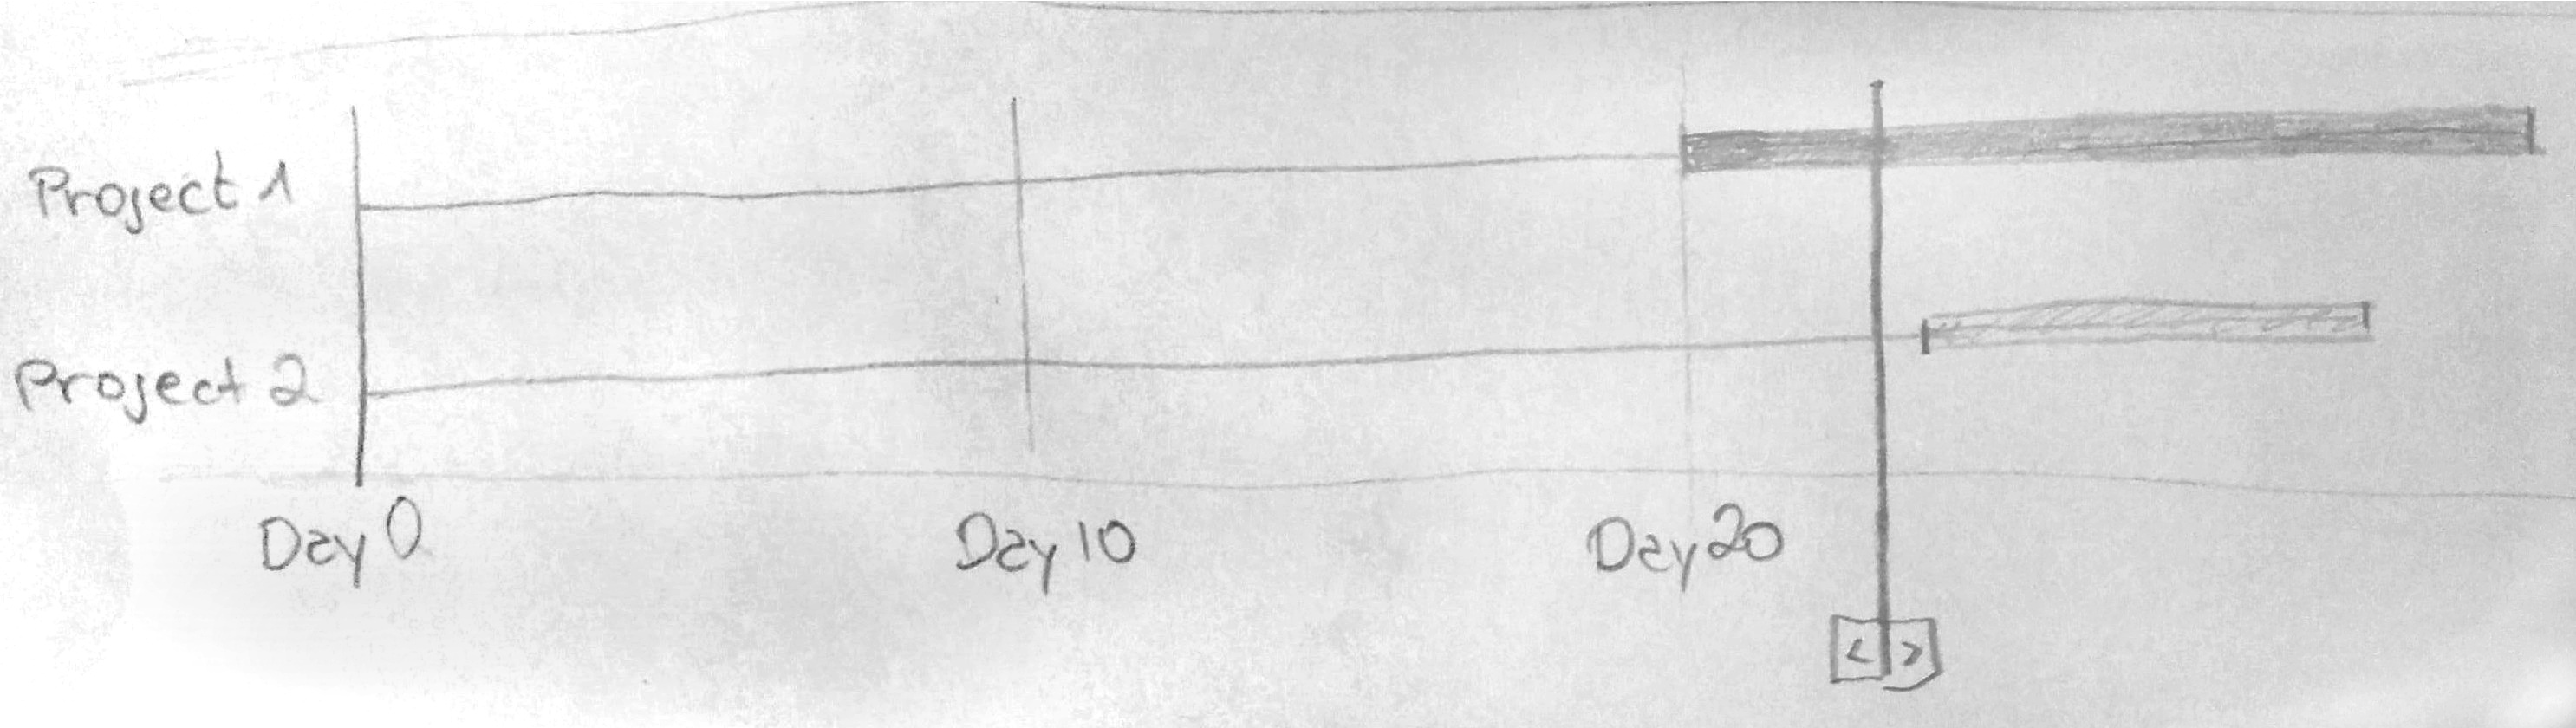
\includegraphics[height=0.3\textwidth]{figures/t2interaction.jpg}
		\caption{\textit{This visualization only shows the bounds of the uncertain time frames, but also shows explicit values through user interaction. The user can slide the slider on the bottom to a specific time point to get information about the respective possibilities of both events.}}
		\label{fig:t2interaction}
	\end{minipage}
\end{figure}


Even though most sketches feature uncertainty in an explicit way, there are still many bounded visualizations. We believe that this is due to our task description. To support the user in the goal of Task 2, only the average value of the two intervals are needed. Hence, there is no need to visualize uncertainty to a given point in time explicitly. The fact that uncertainty was drawn so many times, even though it is not relevant for the task at hand, might be an indication that: \textbf{H8 Most people prefer to have the underlying uncertainty of data presented to them, even if it is not directly relevant for the task at hand.} An example for the additional visualization of uncertainty can be seen in Figure \ref{fig:t2length}.  \par \medskip

Table \ref{tb:t4} shows the results of Task 4. The most apparent difference between these results and the previous ones is that over two thirds of sketches feature the two relevant time intervals in a superimposed view, instead of a juxtaposition. We believe that this is due to the nature of the task. In contrast to the previous scenario, the two intervals are both happening after each other, with the possibility of overlap and there is not direct comparison of the two. \textbf{H9 To represent the amount of overlap between events, it is intuitive to superimpose them in the same view.}\par \medskip

It is also noteworthy that there are more clock metaphors, like the one in Figure \ref{fig:t4clock}, used in this task, compared to the previous ones. We believe that this is because: \textbf{H10 Clocks lend themselves to show two superimposed time intervals, as long as the overlapping area does not exceed a one hour time frame.} \par \medskip

\begin{figure}[H]
	\begin{minipage}{.5\textwidth}
		\centering
		\captionsetup{width=0.8\textwidth}
		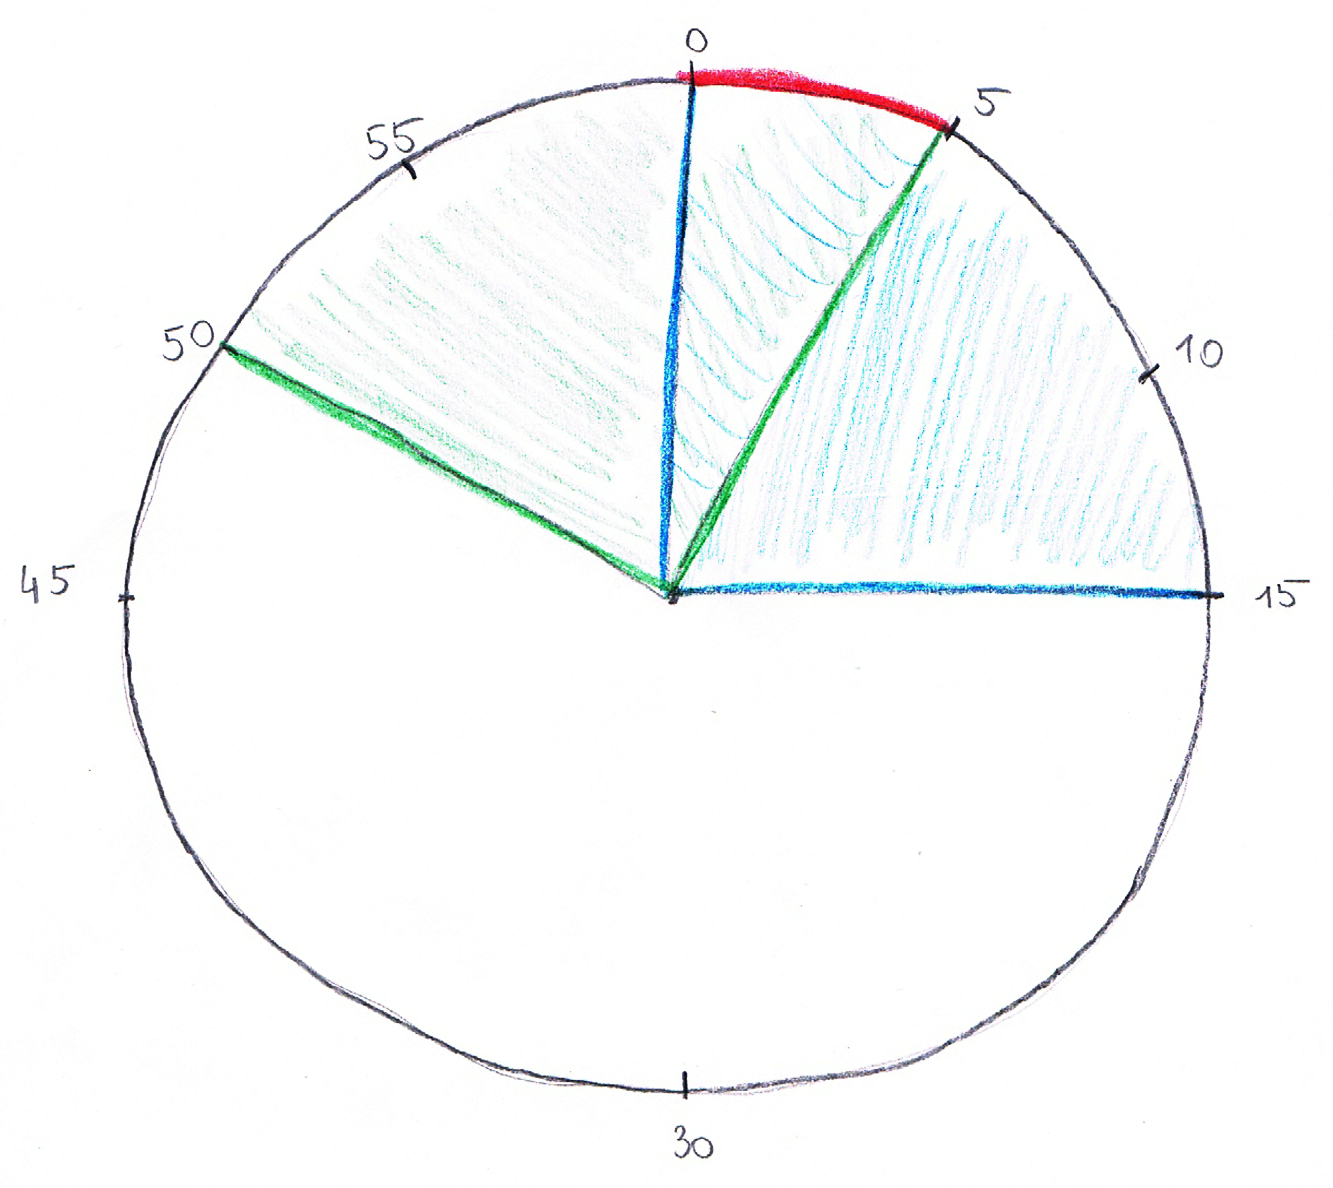
\includegraphics[height=0.6\textwidth]{figures/t4clock.png}
		\caption{\textit{This sketch shows a simple bounded clock visualization. Both uncertainty intervals are colored wedges on the clock. The two colors are mixed within the overlap of the two intervals.}}
		\label{fig:t4clock}
	\end{minipage}
	\begin{minipage}{.5\textwidth}
		\centering
		\captionsetup{width=1.0\textwidth}
		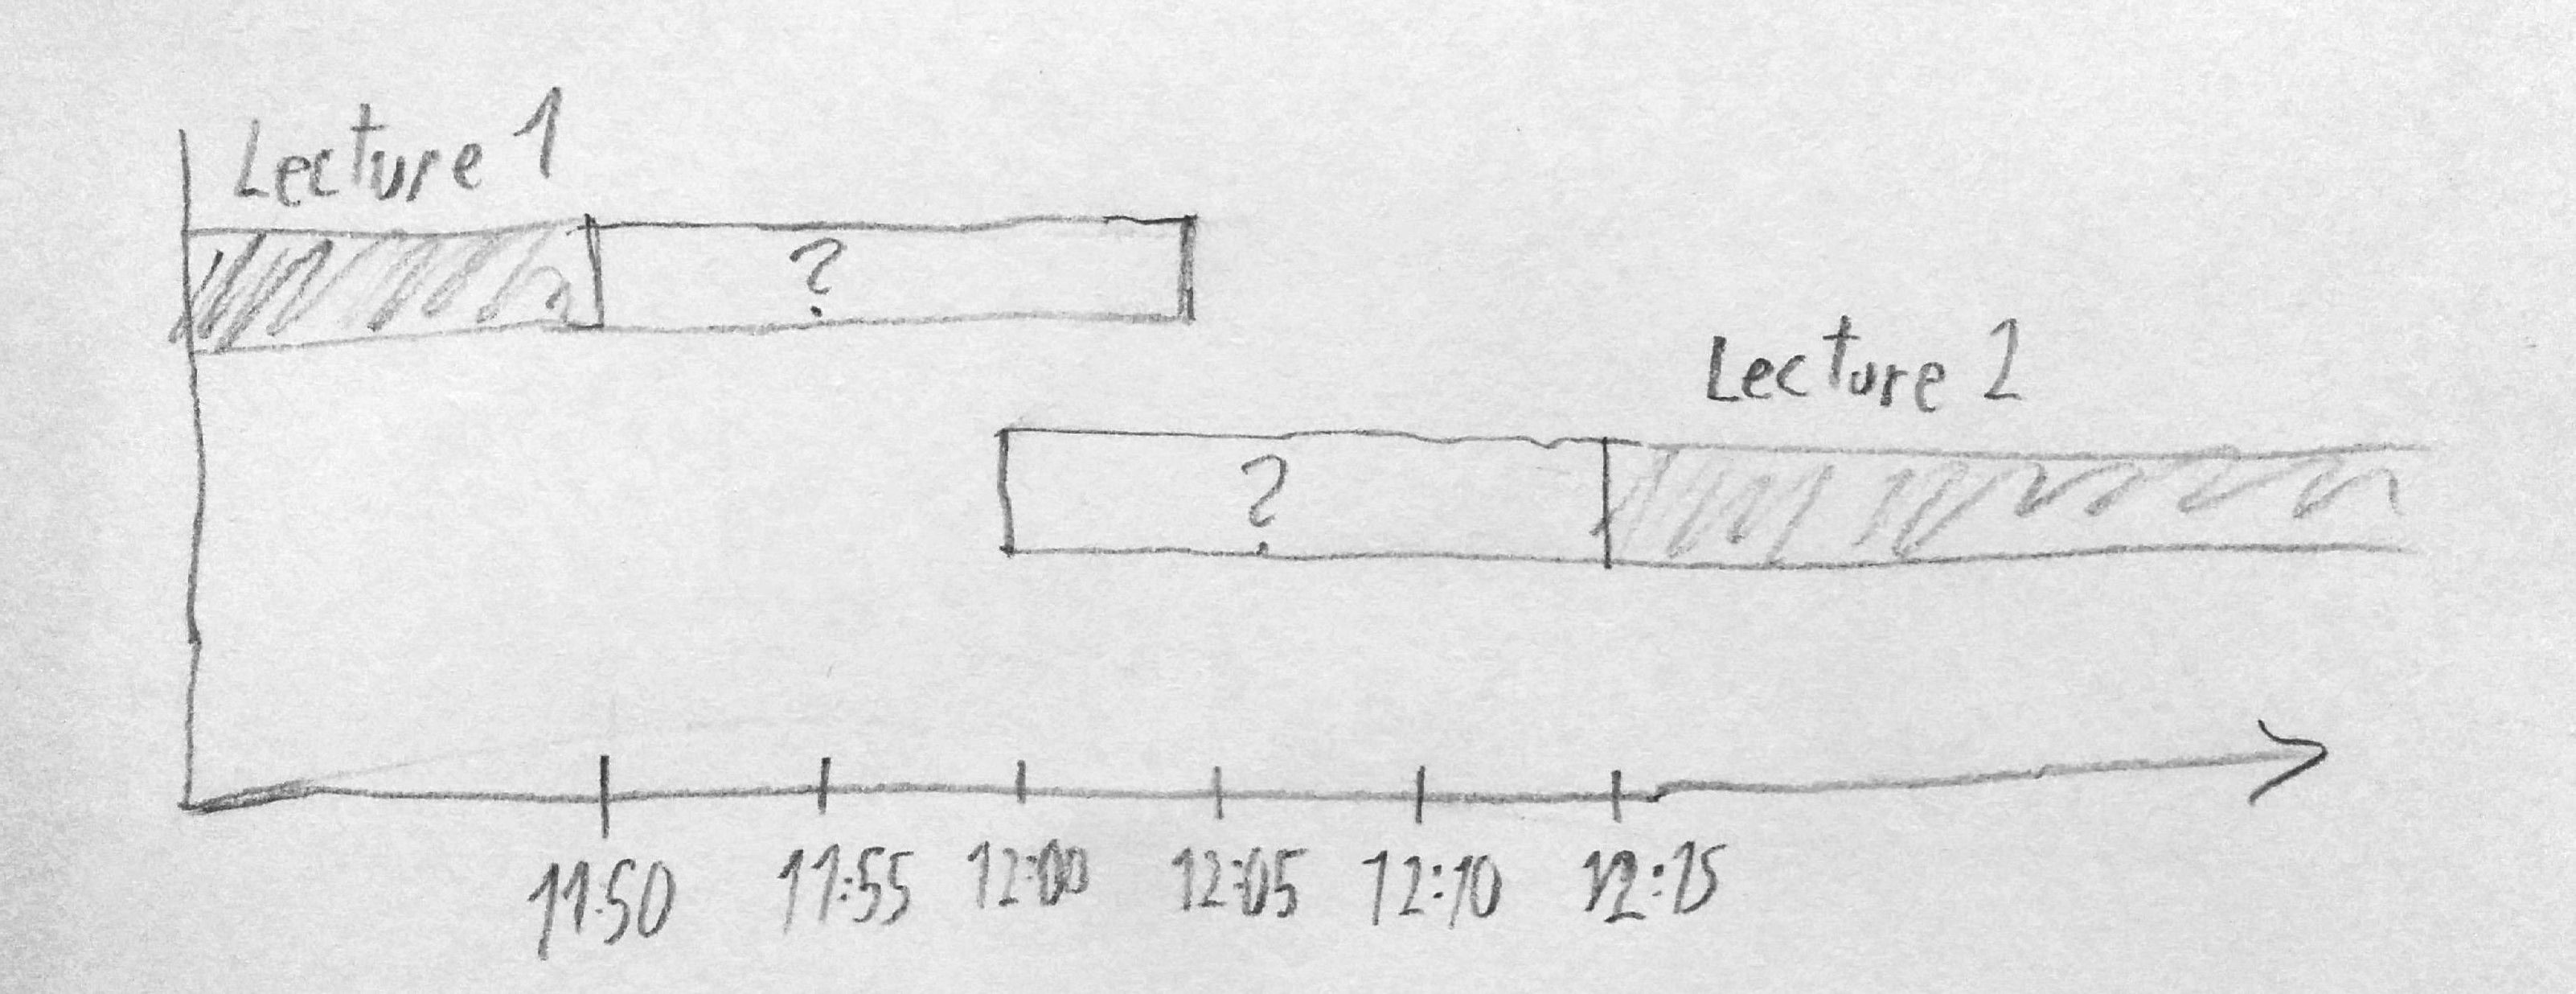
\includegraphics[height=0.4\textwidth]{figures/t4bounded.jpg}
		\caption{\textit{In this sketch both uncertainty intervals are only given by their temporal bounds. The user is not directly supported in figuring out what the possibility of overlap of the two events is.}}
		\label{fig:t4bounded}
	\end{minipage}
\end{figure}

Another significant difference to the last task is the lower amount of explicit uncertainty representations. About two thirds of all sketches of Task 4 are bounded ones, like the one in Figure \ref{fig:t4bounded}. We believe that this is due to the complexity of the underlying goal. It is not trivial to visualize the joint probability of overlap of two intervals. Hence, most people do not have a good idea how to do it and simply visualize the bounds of the two intervals. \textbf{H11 An elaborate way of visualizing the joint probability of two uncertain events, to represent their overlap possibility is not very intuitive for most people.} \par \medskip

Taking a closer look at the sketches that utilize a superposition of the two intervals, shows that half of them use color to distinguish the intervals from each other. The other half does not need color to distinguish them, since they are characterized by their shape or position, like in Figure \ref{fig:t4pos} and \ref{fig:t4shape}. \textbf{H12 Color is an intuitive way of separating two overlapping objects of the same shape.}\par \medskip

\begin{figure}[H]
	\begin{minipage}{.5\textwidth}
		\centering
		\captionsetup{width=0.8\textwidth}
		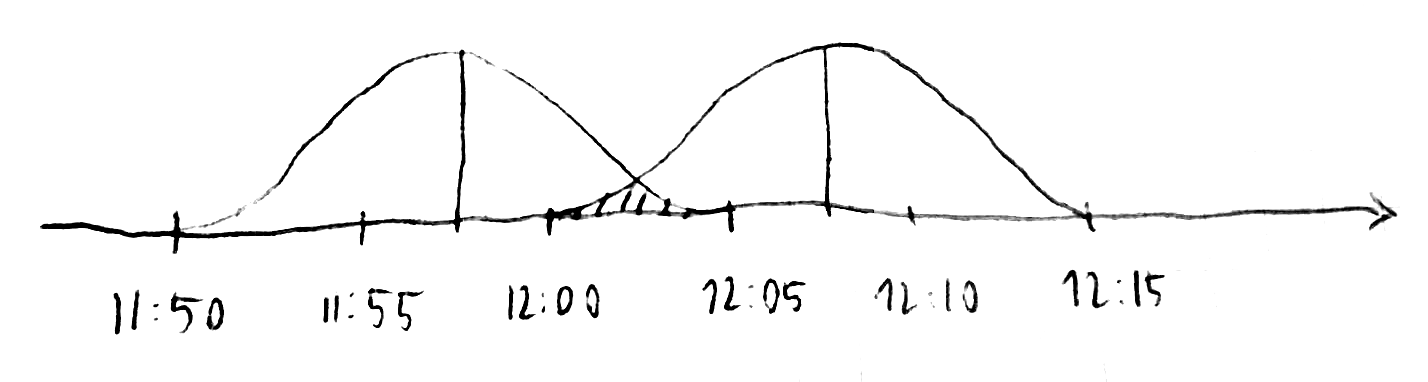
\includegraphics[height=0.28\textwidth]{figures/t4pos.png}
		\caption{\textit{The two graphs, which represent the respective uncertainty intervals of the two events, do not need to be distinguished by color, because they are separated by their position.}}
		\label{fig:t4pos}
	\end{minipage}
	\begin{minipage}{.5\textwidth}
		\centering
		\captionsetup{width=1.0\textwidth}
		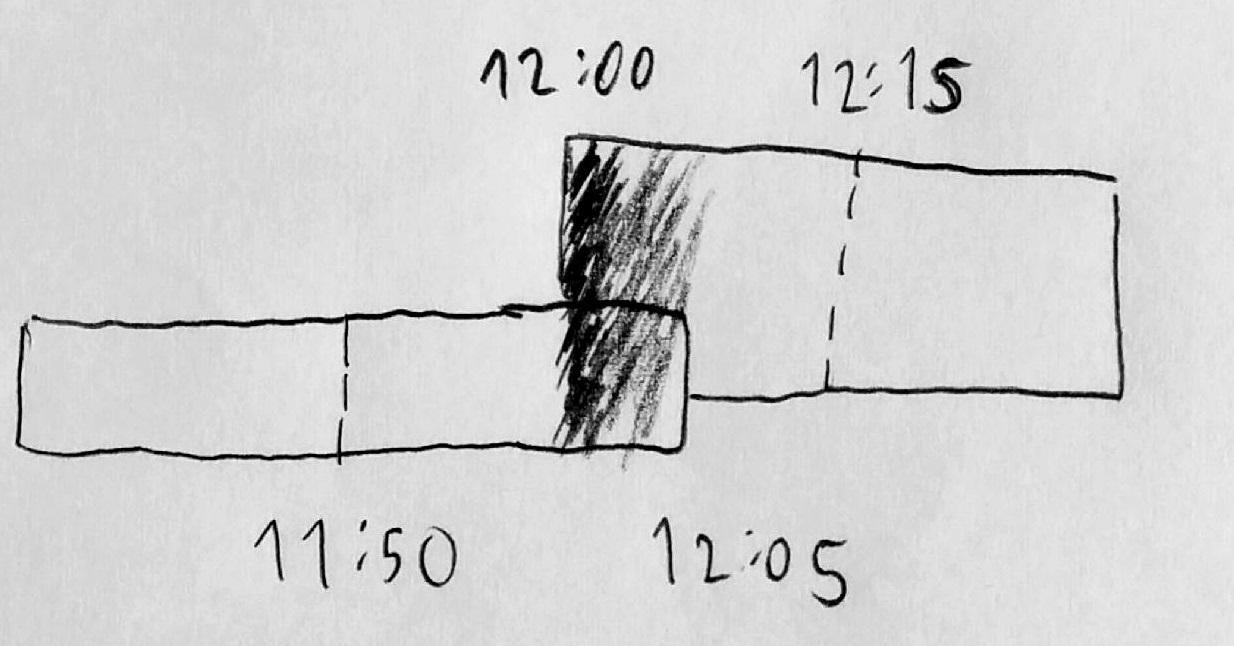
\includegraphics[height=0.45\textwidth]{figures/t4shape.jpg}
		\caption{\textit{In this case the participant used different shapes/sizes for the two uncertainty intervals, which left the color dimension to encode something else than the distinction between the two events.}}
		\label{fig:t4shape}
	\end{minipage}
\end{figure}
